\documentclass[11pt, oneside]{article}   	% use "amsart" instead of "article" for AMSLaTeX format
\usepackage{geometry}                		% See geometry.pdf to learn the layout options. There are lots.
\geometry{letterpaper}                   		% ... or a4paper or a5paper or ... 
%\geometry{landscape}                		% Activate for for rotated page geometry
%\usepackage[parfill]{parskip}    		% Activate to begin paragraphs with an empty line rather than an indent
\usepackage{graphicx}				% Use pdf, png, jpg, or eps� with pdflatex; use eps in DVI mode
								% TeX will automatically convert eps --> pdf in pdflatex		
\usepackage{amssymb}
\usepackage{amsmath}
\usepackage{parskip}

\title{FTC}
%\author{The Author}
%\section{}
% \subsection*{R code}
\date{}							% Activate to display a given date or no date

\graphicspath{{/Users/telliott_admin/Dropbox/Tex/png/}}

\begin{document}
\maketitle
\Large
%\noindent

\begin{center} 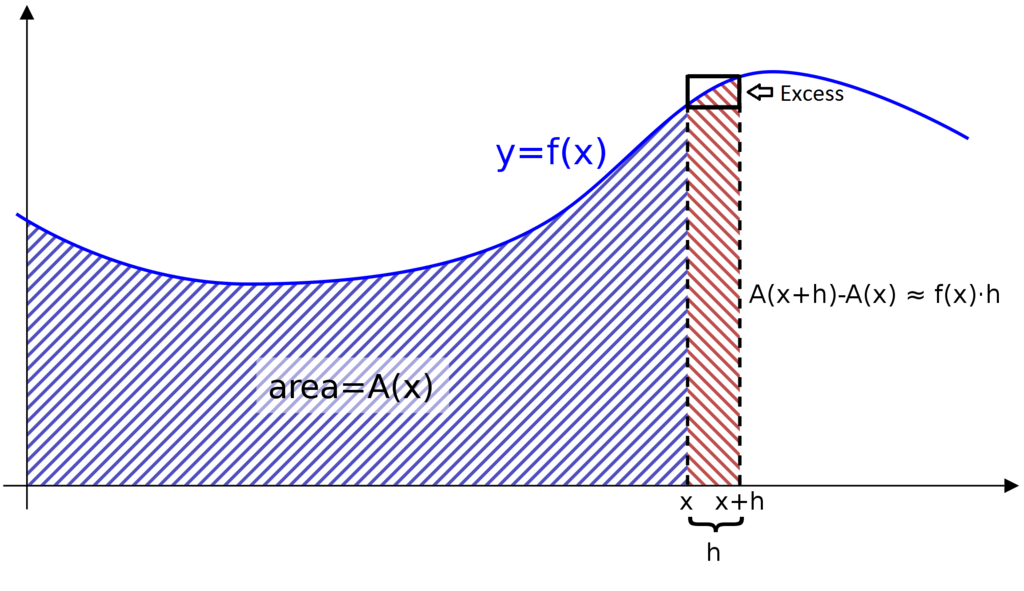
\includegraphics [scale=0.4] {FTC_geometric2.png} \end{center}

The big picture view of the fundamental theorem of calculus (FTC) is that if we consider that the area $A$ under the graph of a function $f(x)$ is itself a function $A(x)$ (having fixed the left-hand boundary for the area), then

\[ A' = f(x) \]

and we can find the area function $A$ as one of the family of \emph{anti-derivatives} of $f$.  

Now, there are conditions, namely that $F$ must be continuous on the interval $[a,b]$ and differentiable on $(a,b)$, and we agree to only look at $x$ values contained in the interval $(a,b)$.  In other words, the function $F$ and its derivative $f$ have to be "nice."  

There are two formal statements of the FTC, that turn out to be equivalent (the second can be proved from the first).

Suppose 
\[ F(x) = \int_a^x f(x) \ dx \]
then
\[ F'(x) = \frac{d}{dx} \ \int_a^x f(x) \ dx = f(x) \]

The expression $\int_a^x f(x) \ dx$ is a \emph{number}, a function of $x$, which gives a different result (usually) for each value of $x$.  Some people use the notation $f(t) \ dt$ so as not to be confused about this.  They will say

\[ F(x) = \int_a^x f(t) \ dt \]
\[ F'(x) = \frac{d}{dx} \ \int_a^x f(t) \ dt = f(x) \]

This is completely equivalent.

The area under the curve $y=f(x)$ betweeen a left-hand boundary $a$ and $x$ grows at the rate $f(x)$.  The derivative of the area function is $f(x)$.

The second version (FTC2) simply gives us a method to calculate what the number is, a way to evaluate integrals:

\[ \int_a^b f(x) \ dx = F(b) - F(a) \]

where $F$ and $f$ are the same as before, namely

\[ F'(x) = f(x) \]
If we can find a function $F$ whose derivative is equal to $f$ then we can evaluate the integral as shown.  An example:
\[ f(x) = x^2 \ dx \]
\[ F(x) = \frac{1}{3}x^3 \]
\[ \int_0^1 x^2 \ dx = \frac{1}{3}x^3 \ \bigg |_0^1 = \frac{1}{3}(1-0) = \frac{1}{3} \]
The area under the curve $f(x) = x^2$ between $x=0 \rightarrow 1$ is just $1/3$.

A simple-minded view of the FTC is that it says that integration and differentiation are the reverse processes for each other.  In fact, this is the fundamental insight of Newton and Leibnitz.

However, it is important to emphasize that the FTC is not the \emph{definition} of integration.  In fact, integration is defined as the limit of Riemann sums of the interval.  What the FTC does is to provide a way process that comes to the same answer as the sum method, but without the pain.

read Bressoud from p. 104 in the AP Calculus handout.

\end{document}  